\documentclass[12pt,]{article}
\usepackage{lmodern}
\usepackage{amssymb,amsmath}
\usepackage{ifxetex,ifluatex}
\usepackage{fixltx2e} % provides \textsubscript
\ifnum 0\ifxetex 1\fi\ifluatex 1\fi=0 % if pdftex
  \usepackage[T1]{fontenc}
  \usepackage[utf8]{inputenc}
\else % if luatex or xelatex
  \ifxetex
    \usepackage{mathspec}
  \else
    \usepackage{fontspec}
  \fi
  \defaultfontfeatures{Ligatures=TeX,Scale=MatchLowercase}
\fi
% use upquote if available, for straight quotes in verbatim environments
\IfFileExists{upquote.sty}{\usepackage{upquote}}{}
% use microtype if available
\IfFileExists{microtype.sty}{%
\usepackage{microtype}
\UseMicrotypeSet[protrusion]{basicmath} % disable protrusion for tt fonts
}{}
\usepackage[margin=1in]{geometry}
\usepackage{hyperref}
\hypersetup{unicode=true,
            pdfauthor={Xuan Son Le (4669361), Freie Universität Berlin},
            pdfborder={0 0 0},
            breaklinks=true}
\urlstyle{same}  % don't use monospace font for urls
\usepackage{color}
\usepackage{fancyvrb}
\newcommand{\VerbBar}{|}
\newcommand{\VERB}{\Verb[commandchars=\\\{\}]}
\DefineVerbatimEnvironment{Highlighting}{Verbatim}{commandchars=\\\{\}}
% Add ',fontsize=\small' for more characters per line
\usepackage{framed}
\definecolor{shadecolor}{RGB}{248,248,248}
\newenvironment{Shaded}{\begin{snugshade}}{\end{snugshade}}
\newcommand{\KeywordTok}[1]{\textcolor[rgb]{0.13,0.29,0.53}{\textbf{#1}}}
\newcommand{\DataTypeTok}[1]{\textcolor[rgb]{0.13,0.29,0.53}{#1}}
\newcommand{\DecValTok}[1]{\textcolor[rgb]{0.00,0.00,0.81}{#1}}
\newcommand{\BaseNTok}[1]{\textcolor[rgb]{0.00,0.00,0.81}{#1}}
\newcommand{\FloatTok}[1]{\textcolor[rgb]{0.00,0.00,0.81}{#1}}
\newcommand{\ConstantTok}[1]{\textcolor[rgb]{0.00,0.00,0.00}{#1}}
\newcommand{\CharTok}[1]{\textcolor[rgb]{0.31,0.60,0.02}{#1}}
\newcommand{\SpecialCharTok}[1]{\textcolor[rgb]{0.00,0.00,0.00}{#1}}
\newcommand{\StringTok}[1]{\textcolor[rgb]{0.31,0.60,0.02}{#1}}
\newcommand{\VerbatimStringTok}[1]{\textcolor[rgb]{0.31,0.60,0.02}{#1}}
\newcommand{\SpecialStringTok}[1]{\textcolor[rgb]{0.31,0.60,0.02}{#1}}
\newcommand{\ImportTok}[1]{#1}
\newcommand{\CommentTok}[1]{\textcolor[rgb]{0.56,0.35,0.01}{\textit{#1}}}
\newcommand{\DocumentationTok}[1]{\textcolor[rgb]{0.56,0.35,0.01}{\textbf{\textit{#1}}}}
\newcommand{\AnnotationTok}[1]{\textcolor[rgb]{0.56,0.35,0.01}{\textbf{\textit{#1}}}}
\newcommand{\CommentVarTok}[1]{\textcolor[rgb]{0.56,0.35,0.01}{\textbf{\textit{#1}}}}
\newcommand{\OtherTok}[1]{\textcolor[rgb]{0.56,0.35,0.01}{#1}}
\newcommand{\FunctionTok}[1]{\textcolor[rgb]{0.00,0.00,0.00}{#1}}
\newcommand{\VariableTok}[1]{\textcolor[rgb]{0.00,0.00,0.00}{#1}}
\newcommand{\ControlFlowTok}[1]{\textcolor[rgb]{0.13,0.29,0.53}{\textbf{#1}}}
\newcommand{\OperatorTok}[1]{\textcolor[rgb]{0.81,0.36,0.00}{\textbf{#1}}}
\newcommand{\BuiltInTok}[1]{#1}
\newcommand{\ExtensionTok}[1]{#1}
\newcommand{\PreprocessorTok}[1]{\textcolor[rgb]{0.56,0.35,0.01}{\textit{#1}}}
\newcommand{\AttributeTok}[1]{\textcolor[rgb]{0.77,0.63,0.00}{#1}}
\newcommand{\RegionMarkerTok}[1]{#1}
\newcommand{\InformationTok}[1]{\textcolor[rgb]{0.56,0.35,0.01}{\textbf{\textit{#1}}}}
\newcommand{\WarningTok}[1]{\textcolor[rgb]{0.56,0.35,0.01}{\textbf{\textit{#1}}}}
\newcommand{\AlertTok}[1]{\textcolor[rgb]{0.94,0.16,0.16}{#1}}
\newcommand{\ErrorTok}[1]{\textcolor[rgb]{0.64,0.00,0.00}{\textbf{#1}}}
\newcommand{\NormalTok}[1]{#1}
\usepackage{graphicx,grffile}
\makeatletter
\def\maxwidth{\ifdim\Gin@nat@width>\linewidth\linewidth\else\Gin@nat@width\fi}
\def\maxheight{\ifdim\Gin@nat@height>\textheight\textheight\else\Gin@nat@height\fi}
\makeatother
% Scale images if necessary, so that they will not overflow the page
% margins by default, and it is still possible to overwrite the defaults
% using explicit options in \includegraphics[width, height, ...]{}
\setkeys{Gin}{width=\maxwidth,height=\maxheight,keepaspectratio}
\IfFileExists{parskip.sty}{%
\usepackage{parskip}
}{% else
\setlength{\parindent}{0pt}
\setlength{\parskip}{6pt plus 2pt minus 1pt}
}
\setlength{\emergencystretch}{3em}  % prevent overfull lines
\providecommand{\tightlist}{%
  \setlength{\itemsep}{0pt}\setlength{\parskip}{0pt}}
\setcounter{secnumdepth}{5}
% Redefines (sub)paragraphs to behave more like sections
\ifx\paragraph\undefined\else
\let\oldparagraph\paragraph
\renewcommand{\paragraph}[1]{\oldparagraph{#1}\mbox{}}
\fi
\ifx\subparagraph\undefined\else
\let\oldsubparagraph\subparagraph
\renewcommand{\subparagraph}[1]{\oldsubparagraph{#1}\mbox{}}
\fi

%%% Use protect on footnotes to avoid problems with footnotes in titles
\let\rmarkdownfootnote\footnote%
\def\footnote{\protect\rmarkdownfootnote}

%%% Change title format to be more compact
\usepackage{titling}

% Create subtitle command for use in maketitle
\newcommand{\subtitle}[1]{
  \posttitle{
    \begin{center}\large#1\end{center}
    }
}

\setlength{\droptitle}{-2em}
  \title{\textbf{Logistische Regression}}
  \pretitle{\vspace{\droptitle}\centering\huge}
  \posttitle{\par}
  \author{Xuan Son Le (4669361), Freie Universität Berlin}
  \preauthor{\centering\large\emph}
  \postauthor{\par}
  \predate{\centering\large\emph}
  \postdate{\par}
  \date{02/04/2018}

\usepackage{caption}
\captionsetup[figure]{name=Abbildung}

\begin{document}
\maketitle

\begin{center}\rule{0.5\linewidth}{\linethickness}\end{center}

\textbf{Abstract}: Im Rahmen der Abschlussarbeit des Moduls
Programmieren mit R im Wintersemester 2017/2018 an der Freie Universität
Berlin wird für diese Arbeit die statistische Methode namens binäres
Logit-Modell ausgewählt. Diese Arbeit besteht aus zwei großen
Hauptteilen: der Theorieteil, wobei die ausgewählte Methode theoretisch
vorgestellt wird und der Implementierungsteil, welcher die Erklärung der
Funktionalität vom selbst entwickelten Paket beinhaltet. Im Theorieteil
wird zunächst die Grundidee von Generalisierten Linearen Modellen (GLMs)
widergegeben. Anschließend werden die grundliegende Funktionsweise vom
(binären) Logit-Modell sowie dessen Aufbau durch das Maximum Likelihood
Verfahren vorgenommen. Demzufolge folgt die Interpretation der
Koeffizienten vom binären Logit-Modell. Schließlich werden im
Implementierungsteil alle Funktionen vom R-Paket schritterweise
vorgestellt.

\textbf{Keywords:} \emph{Logit-Modell, logistische Regression, R-Paket,
Maximum Likelihood}

\begin{center}\rule{0.5\linewidth}{\linethickness}\end{center}

\newpage

\section{Motivation}\label{motivation}

Die Anwendung von der klassischen linearen Regression ist für binäre
(binomiale oder dichotome) Zielvariable (Response- oder zu erklärende
Variable), welche lediglich zwei Werte (ja/nein, mänlich/weiblich,
erfolgreich/nicht erfolgreich, etc.) annehmen kann, nicht mehr geeignet,
da die Zielvariable von der linearen Regression metrisch skaliert ist.
Oft wird binäre Variable als 0/1-Variable kodiert, das heißt sie nimmt
nur den Wert 0 oder 1 an. Abbildung 1 stellt den Ansatz graphisch dar,
binäre Variable durch lineare Regression zu modellieren:

\begin{figure}[h]

{\centering 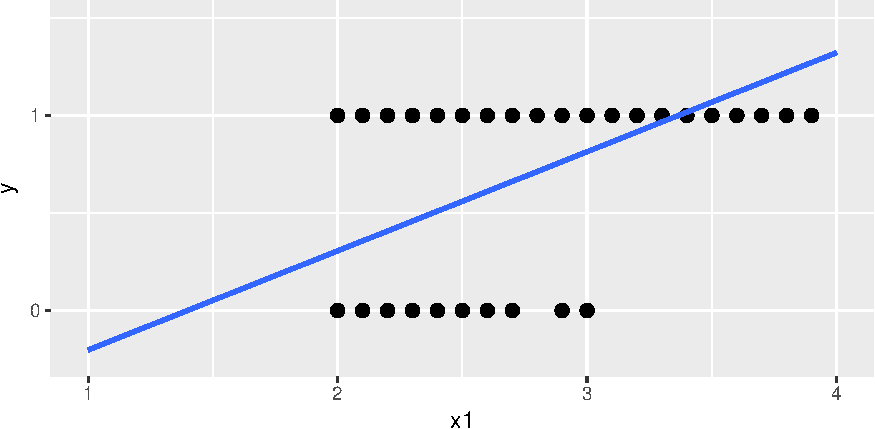
\includegraphics{logisticRegression_files/figure-latex/unnamed-chunk-1-1} 

}

\caption{Beispielshafte lineare Regression für binäre Zielvariable}\label{fig:unnamed-chunk-1}
\end{figure}

Graphisch lässt sich festlegen, dass die lineare Regression den
Wertebereich {[}0,1{]} von binären Responsevariablen sehr schnell
verlässt. Aus diesem Grund wird ein ganz anderer Ansatz benötigt, um
binäre Zielvariable zu modellieren, nämlich das binäre Logit-Modell
(auch binäre logistische Regression oder binäres logistisches
Regressionsmodell). In der Statistik lassen sich Logit-Modelle noch in
multinomiale und kumulative Logit-Modelle aufteilen, je nachdem ob die
abhängige Variable multinominal- oder ordinalskaliert sind (vgl.
Schlittgen
(\protect\hyperlink{ref-schlittgen2013regressionsanalysen}{2013}), S.225
ff.). Diese Arbeit beschäftigt sich mit dem binären Logit-Modell,
welches den Zusammenhang zwischen einer binären abhängigen Variable und
einer/mehreren unabhängigen Variablen untersucht. Bei allen Arten von
Logit-Modellen können die unabhängigen Variablen (erklärende oder
Kovariablen) beliebig skaliert sein.

Im Unterschied zu der klassischen linearen Regression, welche den wahren
Wert einer Zielvariable vorhersagt, interessiert sich das binäre
Logit-Modell eher für die Wahrscheinlichkeit, dass die Zielvariable den
Wert 1 annimmt. Das Hauptziel vom binären Logit-Modell ist es, die
Wahrscheinlichkeit für den Eintritt der Zielvariable vorherzusagen.
Dadurch soll die folgende theoretische Fragestellung beantwortet werden:
\emph{Wie stark ist der Einfluss von den unabhängigen (erklärenden)
Variablen auf die Wahrscheinlichkeit, dass die abhängige (zu erklärende
/ Response) Variable eintritt beziehungsweise den Wert 1 annimmt?} In
der Praxis kann diese Fragestellung beispielsweise so formuliert werden:
``Haben Alter, Geschlecht, Berufe oder andere Merkmale der Kunden
Einfluss auf die Wahrscheinlichkeit, dass sie ein Kredit rechtzeitig
zurückzahlen?'' oder ``Lässt sich die Wahrscheinlichkeit, dass es
regnet, durch die Temparatur, die Windstärke oder
Sonnenstrahlungsintensität vorhersagen?''. \newpage 

\section{Das binäre Logit-Modell}\label{das-binare-logit-modell}

Das Logit-Modell ist eine Methode aus der Algorithmenklasse namens
\emph{Generalisierte Lineare Modelle} (engl. generalized linear model,
kurz GLM), welche eine Verallgemeinerung des klassischen linearen
Regressionsmodells anstrebt. Dazu gehören noch die klassische lineare
Regression, Probitmodell und Poisson-Regression. Der grundliegende
Ansatz von GLM ist die Transformation der linearen Regressionsgleichung,
so dass der Wertebereich der vorhergesagten Zielvariable dem gewünschten
entspricht. Die Theorie von GLMs wurde von Nelder und Wedderburn
entwickelt. In Anlehnung an Schlittgen
(\protect\hyperlink{ref-schlittgen2013regressionsanalysen}{2013}), S.238
können Modelle zu GLMs zugeordnet werden, wenn:

\begin{enumerate}
\def\labelenumi{\arabic{enumi}.}
\tightlist
\item
  der bedingte Erwartungswert von der abhängigen Variable \(y_i\),
  \(\mu_i = E(y_i|x_i)\), kann über eine Linkfunktion
  \(\mathbf{g}(\mu_i)\) in eine lineare Kombination der unabhängigen
  Variablen transformiert werden:
  \[\mathbf{g}(\mu_i) = \eta_i = x_i.\beta\] Wird die Umkehrfunktion
  gebildet, ergibt sich die Responsefunktion, welche die Abhängigkeit
  der Erwartungswerte von einer Funktion des linearen Prädikators
  darstellt:
  \[\mu_i = \mathbf{g}^{-1}(\eta_i) = \mathbf{h}(\eta_i) =  \mathbf{h}(\mathbf{g}(\mu_i))
  \]
\item
  Die abhängige Variable gehört zu einer Exponentialfamilie mit der
  Dichtefunktion: \[
  f(y_i;\theta_i) = \exp \Bigg( \frac{y_i.\theta_i + b(\theta_i)}{a_i(\phi)} + c(y,\phi) \Bigg)
  \]
\end{enumerate}

Die mathematische Erklärung von GLMs wird hierbei vernachlässigt, denn
diese Arbeit konzentriert sich lediglich auf dem binären Logit-Modell,
welches in Folgenden vorgestellt werden.

\subsection{Modellspezifikation}\label{modellspezifikation}

Die folgende Modellspezifikation vom binären Logit-Modell basiert sich
auf Kapitel 9.1 aus dem Buch \emph{Regressionsanalysen mit R}
(Schlittgen,
\protect\hyperlink{ref-schlittgen2013regressionsanalysen}{2013},
S.215-225) und Kapitel 4.1 der Vorlesungsfolien vom Modul
\emph{Statistische Modellierung} im Wintersemester 2016/2017 an der
Freie Universität Berlin.

Gegeben seien n unabhängige Beobachtungen \(y_1, y_2, ...,y_n\) der
binären Zielvariable \(\mathbf{Y}\). Ein Verteilungsmodell für
\(\mathbf{Y}\) ist die Binomialverteilung:
\(\mathbf{Y}_i \sim B(1, \pi_i)\) mit \(\pi_i = P(Y_i = 1)\). Für diese
Arbeit wird \(\pi_i = (\pi_1, \pi_2, ..., \pi_n)\) als die
Eintrittwahrscheinlichkeit von der einzelnen \(\mathbf{Y}_i\) benannt.
Weiterhin seien p erklärende Variablen
\(\mathbf{X}_0,\mathbf{X}_1,..,\mathbf{X}_p\) gegeben mit jeweils n
unabhängigen Beobachtungen
\(\mathbf{X}_j = (x_{1j}, x_{2j},..., x_{nj})\) mit j \(\in\)
\{0,1,2,..,p\} - gegeben. Daraus ergeben sich p Koeffizienten
\(\beta = (\beta_0, \beta_1, \beta_2,..., \beta_p)\), welche die Stärke
den Zusammenhang zwischen die einzelne erklärende Variable mit der
Zielvariable widerspiegeln. Dabei ist es sinnvoll, diese in einer
Designmatrix \(\mathbf{X}\) zu speichern. Da der Interzept (\(\beta_0\))
ebenfalls geschätzt werden soll, sind alle Werte der ersten Spalte von X
gleich Eins, also \(x_{10} = x_{20} = ... = x_{n0} = 1\).
Zusammengefasst lässt sich die Designmatrix wie folgt darstellen: \[
\mathbf{X} =
 \begin{pmatrix}
    1 & x_{11} & x_{12} & \cdots & x_{1p} \\
    1 & x_{21} & x_{22} & \cdots & x_{2p} \\
    1 & x_{31} & x_{32} & \cdots & x_{3p} \\
    \vdots  & \vdots  & \vdots & \ddots & \vdots \\
    1 & x_{n1} & x_{n2} & \cdots & x_{np}
 \end{pmatrix}
\] Die dazugehörige lineare Regressionsgleichung lautet:
\(\mathbf{Y} = \mathbf{X}.\beta + \epsilon\) mit
\(\epsilon = (\epsilon_1, \epsilon_2, \epsilon_3, ..., \epsilon_n)\) als
die Abweichung der einzelnen Schätzungen gegenüber dem wahren Wert,
wobei \(\mathbf{Y}\) ein (nx1)-Vektor, \(\mathbf{X}\) ein (nxp) und
\(\beta_i\) sowie \(\epsilon_i\) ein (px1)-Vektor ist.

Die einzelne Beobachtung lässt sich wie folgt darstellen: \[
y_i = \beta_0 + \beta_1.x_{i1} + \beta_2.x_{i2} + ... + \beta_p.x_{ip} + \epsilon_i = \mathbf{x'}_i.\beta + \epsilon_i \qquad \forall_i = 1,2,3,...,n
\] Wobei \(\mathbf{x}_i\) der i-ten Zeile der Designmatrix
\(\mathbf{X}\) entspricht. Da bei der Multiplikation A.B die Regel gilt,
dass die Spaltenanzahl von A der Zeilenanzahl von B entsprechen muss. Da
\(\beta\) ein (px1)-Vektor ist, muss \(\mathbf{x}_i\) (px1-Vektor) in
\(\mathbf{x'}_i\) (1xp-Vektor) transponiert werden, damit die
Multiplikation durchführbar ist.

Um die Werte im Bereich der reellen Zahlen von der linearen Regression
auf dem Wertebereich von Wahrscheinlichkeiten zwischen 0 und 1 zu
beschränken, sollte die rechte Seite der Gleichung transformiert werden.
Das Ziel ist es, eine sinnvolle Verteilungsfunktion (Responsefunktion)
zu finden, deren Wertebereich in {[}0,1{]} liegt:
\(\pi_i = P(\mathbf{Y_i} = 1) = F(\beta_0 + \beta_1.x_{i2} + \beta_2.x_{i3} + ... + \beta_p.x_{ip}) = F(\eta_i)\).
Der lineare Prädikator
\[\eta_i = \beta_0 + \beta_1.x_{i2} + \beta_2.x_{i3} + ... + \beta_p.x_{ip} = \mathbf{x'}_i.\beta \ \ (1)\]
wird ebenfalls als Linkfunktion genannt, weil dadurch eine Verbindung
(Link) zwischen der Eintrittwahrscheinlichkeit und den unabhängigen
Variablen erfolgt wird. Für das binäre Logit-Modell wird anstelle der
Responsefunktion die standardisierte logistische Verteilung verwendet:
\[
F(\eta_i) = Logist(\eta_i) = \frac{\exp(\eta_i)}{1 + \exp(\eta_i)} \quad (2)
\]

Da durch die Responsefunktion die Eintrittwahrscheinlichkeit \(\pi_i\)
modelliert werden soll, ergibt sich die Gleichung für das binäre
Logit-Modell wie folgt: \[
\pi_i = h(\eta_i) = \frac{\exp(\eta_i)}{1 + \exp(\eta_i)} = \frac{\exp(\mathbf{x'}_i.\beta)}{1+\exp(\mathbf{x'}_i.\beta)} \quad (3)
\]

Dabei kann \(\pi_i\) maximal den Wert 1 nehmen, wenn \(\exp(\eta_i)\)
sehr groß ist und minimal den Wert 0, wenn \(\exp(\eta_i)\) sehr nah
rechts von 0 liegt. \(\exp(\eta_i)\) kann nicht negativ sein. Diese
Gleichung erfüllt somit die Anforderung bezüglich dem Wertebereich von
Wahrscheinlichkeiten.

Soll die Gleichung nach dem linearen Prädikator \(\eta_i\) gelöst
werden, ergibt sich schließlich die Logit-Linkfunktion: \[
\begin{aligned}
\pi_i.(1 + \exp(\eta_i)) &= \exp(\eta_i) \\
\Leftrightarrow \pi_i + \pi_i.\exp(\eta_i) &= \exp(\eta_i) \\
\Leftrightarrow \pi_i &= \exp(\eta_i) - \pi_i.\exp(\eta_i)  \\
\Leftrightarrow \pi_i &= \exp(\eta_i).(1-\pi_i) \\
\Leftrightarrow \exp(\eta_i) &= \frac{\pi_i}{1-\pi_i} \\
\Leftrightarrow \eta_i &= \ln(\frac{\pi_i}{1-\pi_i}) \quad (4)\\
\end{aligned} 
\]

Schlittgen
(\protect\hyperlink{ref-schlittgen2013regressionsanalysen}{2013}),
S.236-237 zeigt, dass die Wahrscheinlichkeitsfunktion vom binären
Logit-Modell sich mit der Exponentialfunktion schreiben lässt. Somit
erfüllt das binäre Logit-Modell alle Anforderungen für ein GLM.

\subsection{Maximum Likelihood
Schätzung}\label{maximum-likelihood-schatzung}

Ähnlich wie bei der linearen Regression müssen bei dem binären
Logit-Modell die unbekannten Parameter \(\beta_i\) (i =
0,1,2,\ldots{},k) ebenfalls geschätzt werden. Bei der klassischen
linearen Regression wird die Methode der Kleinsten Quadrate (engl.
\emph{method of least squares}, kurz KQ-Methode) genutzt, um eine
Regressionslinie zu bestimmen, welche die Summe der quadratischen
Abweichungen von den beobachteten Punkten minimiert. Da bei dem binären
Logit-Modell nicht der wahre Wert der Zielvariable sondern die
Eintrittswahrscheinlichkeit geschätzt wird, ist die direkte Abweichung
zwischen dem wahren Wert (0/1-Variable) und dem geschätzten Wert
(Wahrscheinlichkeit) nicht mehr aussagekräftig wie bei der linearen
Regression. Die Koeffizienten müssen anders geschätzt werden.
Dementsprechend wird bei dem binären Logit-Modell die sogenannte Maximum
Likelihood Schätzung (kurz ML-Schätzung) eingesetzt. Abbildung 2 zeigt
ein Beispiel mit zwei mögliche binäre logistiche Regressionskurven, die
durch das Maximum Likelihood optimiert werden sollen. Es gibt unendlich
viele solche Kurven. Das Ziel ist es, die Kurve mit dem höchsten Maximum
Likelihood herauszufinden.

\begin{figure}[h]

{\centering 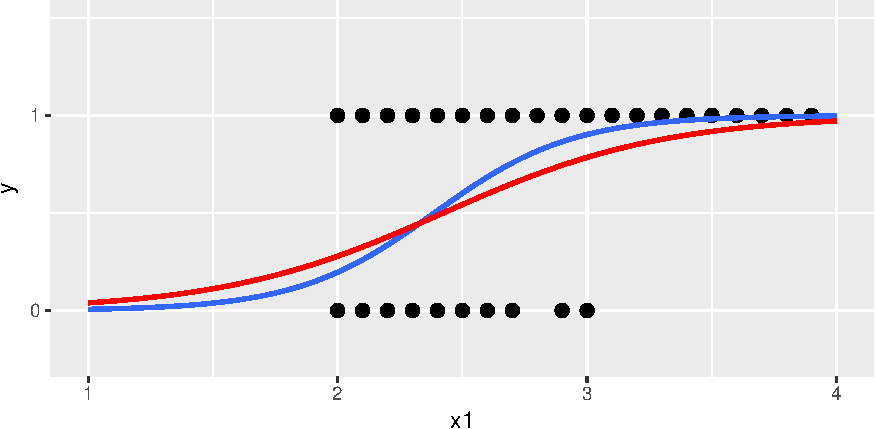
\includegraphics{logisticRegression_files/figure-latex/unnamed-chunk-2-1} 

}

\caption{Beispielshafte logistische Regressionskurve}\label{fig:unnamed-chunk-2}
\end{figure}

Das Ziel der ML-Schätzung besteht darin, die Eintrittswahrscheinlichkeit
für die empirischen Beobachtungswerte zu maximieren. Dafür kommt die
(Log-)Likelihood-Funktion zum Einsatz. Im Folgenden wird die
Vorgehensweise zum Lösen der ML-Schätzung anhand der
Log-Likelihood-Funktion wiedergegeben:

\begin{enumerate}
\def\labelenumi{\arabic{enumi}.}
\tightlist
\item
  Maximum Likelihood Funktion
\item
  Log-Likelihood-Funktion
\item
  Score-Funktion (erste Ableitung)
\item
  Hesse Matrix (zweite Ableitung)
\item
  Newton-Raphson-Methode
\end{enumerate}

\subsubsection{Maximum Likelihood
Funktion}\label{maximum-likelihood-funktion}

Gegeben sei \(y_i = 1\) mit der Eintrittswahrscheinlichkeit \(\pi_i\),
und \(y_i = 0\) mit der Gegenwahrscheinlichkeit \((1-\pi_i)\). Die
Likelihood-Funktion lässt sich wie folgt definieren: \[
\mathcal{L}(\beta) = {\prod_{i=1}^{n} \pi_i^{y_i}.(1-\pi_i)^{1-y_i}} \quad (6)
\] Wenn \(y_i\) gleich 1 ist, ergibt sich für die betroffene Beobachtung
die Eintrittswahrscheinlichkeit \(\pi_i\) und umgekehrt. Das Likelihood
ist gleich die Multiplikation der Wahrscheinlichkeiten von allen
Beobachtungen. Dieses soll maximiert werden.

Da \(\pi_i\) von dem linearen Prädikator \(\eta_i\) abhängt, ist die
Likelihood-Funktion von \(\beta\) abhängig. Wird
\(\pi_i = \frac{\exp(\eta_i)}{1 + \exp(\eta_i)}\) in die
Likelihood-Funktion eingesetzt, ergibt sich:

\[
\mathcal{L}(\beta) = {\prod_{i=1}^{n} \Bigg[ \Big( \frac{\exp(\eta_i)}{1 + \exp(\eta_i)} \Big)^{y_i}.\Big(1-\frac{\exp(\eta_i)}{1 + \exp(\eta_i)}\Big)^{1-y_i}}\Bigg] \quad (7)
\]

\subsubsection{Log-Likelihood-Funktion}\label{log-likelihood-funktion}

Der Versuch, Gleichung (7) zu differenzieren und nach \(\beta\) zu
lösen, um die Extremwerte zu finden, ist extrem aufwendig, weil sie eine
Serie von Multiplikationen enthält. Wegen den exponentialen Komponenten
kann die logistische Funktion aus der Mathematik zur Vereinfachung der
Likelihood-Funktion Einsatz finden. Da die logistische Funktion eine
monotone Funktion ist, entspricht jedes Maximum von der
Likelihood-Funktion dem Maximum von der Log-Likelihood-Funktion und
umgekehrt. Es gelgen für den Logarithmus folgende Regelungen (seien alle
Vorzeichenvoraussetzungen für den Logarithmus erfüllt): \[
\begin{aligned}
(8) \quad &\ln(\prod_{i=1}^{n}x_i) = \ln(x_1.x_2...x_n) = \ln(x_1) + \ln(x_2) + \ ... \ + \ln(x_n) = \sum_{i=1}^{n} \ln(x_i) \\
(9) \quad &\ln(x^\alpha) = \alpha.\ln(x) \\
(10) \quad &\ln(\frac{x}{y}) = \ln(x) - \ln(y)
\end{aligned} 
\] Dementsprechend lässt die Log-Likelihood-Funktion wie folgt
logarithmisieren: \[
\begin{aligned}
\ell(\beta) = \ln(\mathcal{L}(\beta)) = \quad &\ln \Bigg( \prod_{i=1}^{n} \pi_i^{y_i}.(1-\pi_i)^{1-y_i} \Bigg) \\
\mathrel{\overset{(8)}{=}} \quad &\sum_{i = 1}^{n} \ln \Big(\pi_i^{y_i}.(1-\pi_i)^{1-y_i}\Big) \\
\mathrel{\overset{(9)}{=}} \quad &\sum_{i = 1}^{n} \Big( y_i.\ln(\pi_i) + (1-y_i).\ln(1-\pi_i) \Big) \\
= \quad &\sum_{i = 1}^{n} \Big( y_i.\ln(\pi_i) - y_i.\ln(1-\pi_i) + \ln(1-\pi_i) \Big) \\
\mathrel{\overset{(10)}{=}} \quad &\sum_{i = 1}^{n} \Bigg( y_i.\ln \Big(\frac{\pi_i}{1-\pi_i}\Big) + \ln(1-\pi_i) \Bigg) \\
\mathrel{\overset{(4),(3)}{=}} \ &\sum_{i = 1}^{n} \Bigg( y_i.\eta_i + \ln \Big( 1- \frac{\exp(\eta_i)}{1 + \exp(\eta_i)} \Big) \Bigg) \\
= \quad &\sum_{i = 1}^{n} \Bigg( y_i.\eta_i + \ln \Big( \frac{1}{1+\exp(\eta_i)}\Big) \Bigg) \\
= \quad &\sum_{i = 1}^{n} \Big( y_i.\eta_i - \ln (1 + exp(\eta_i)) \Big) \quad (11)
\end{aligned}
\]

\subsubsection{Score-Funktion}\label{score-funktion}

Zum Herausfinden des ML-Schätzers, welcher die log-Likelihood-Funktion
optimiert, wird Gleichung (10) nach \(\beta\) differenziert. Die erste
Ableitung von der log-Likelihood-Funktion wird als Score-Funktion
benannt:

\[
\begin{aligned}
s(\beta) = \frac{\partial}{\partial \beta}  \ell(\beta) &= \frac{\partial}{\partial \beta} \sum_{i = 1}^{n} \Big( y_i.\eta_i - \ln (1 + \exp(\eta_i)) \Big) \quad \\
&\mathrel{\overset{(1)}{=}} \frac{\partial}{\partial \beta} \sum_{i = 1}^{n} \Big( y_i.\mathbf{x'}_i.\beta  - \ln (1 + \exp(\mathbf{x'}_i.\beta )) \Big) \quad \\ 
\end{aligned}
\]

Seien alle Vorzeichnenanforderungen erfüllt, gelten folgende Regelungen
bezüglich der Differenzierungsrechnung: \[
\begin{aligned}
&(12) \frac{\partial}{\partial t} a.f(t) = (a.f(t))' = a.f'(t) \\
&(13) \frac{\partial}{\partial t} \ln(f(t)) = [\ln(f(t))]' = \frac{f'(t)}{f(t)} \\ 
&(14) \frac{\partial}{\partial t} \exp(f(t)) = [\exp(f(t))]' = f'(t).\exp(f(t)) \\
\end{aligned}
\]

Eingesetzt in die Score-Funktion: \[
\begin{aligned}
s(\beta) &= \sum_{i = 1}^{n} \Bigg( y_i.\mathbf{x'}_i - \frac{\mathbf{x'}_i.\exp(\mathbf{x'}_i.\beta)}{1 + \exp(\mathbf{x'}_i.\beta)} \Bigg) \\
&\mathrel{\overset{(1)}{=}}\sum_{i = 1}^{n} \Bigg[ \mathbf{x'}_i \Bigg( y_i - \frac{\exp(\eta_i)}{1 + \exp(\eta_i)} \Bigg) \Bigg] \\
&\mathrel{\overset{(2)}{=}}  \sum_{i = 1}^{n} \ \mathbf{x'}_i ( y_i - \pi_i) \quad  \\
&= \mathbf{X}'.(y-\pi) \quad (15) 
\end{aligned}
\]

\subsubsection{Hesse Matrix}\label{hesse-matrix}

Da \(s(\beta)\) wegen exponentiellen Komponenten nicht linear von
\(\beta\) abhängt, wird zur Maximierung der Funktion ein iteratives
Verfahren verwendet. Für diese Arbeit wird die Newton-Raphson-Methode
(vgl. \ldots{}) ausgewählt. Dafür muss die zweite Ableitung der Funktion
noch gebildet werden, welche als Hesse-Matrix (H) bezeichnet wird:

\[
\begin{aligned}
\frac{\partial^2}{\partial \beta^2} \ell(\beta) = \frac{\partial}{\partial \beta} s(\beta) = H(\beta) &\mathrel{\overset{(15)}{=}} \frac{\partial}{\partial \beta} \sum_{i = 1}^{n} \ (\mathbf{x'}_i.y_i - \mathbf{x'}_i.\pi_i) \\
&= - \sum_{i = 1}^{n} \Bigg( \mathbf{x'}_i \ .  \Big(\frac{\partial}{\partial \beta} \pi_i \Big) \Bigg) \\
&\mathrel{\overset{(3)}{=}} - \sum_{i = 1}^{n} \Bigg( \mathbf{x'}_i \ .  \Big(\frac{\partial}{\partial \beta} \frac{\exp(\mathbf{x'}_i.\beta)}{1+\exp(\mathbf{x'}_i.\beta)} \Big) \Bigg) \\
\end{aligned}
\]

Wegen \[
\frac{\partial}{\partial t} \frac{f(t)}{g(t)} = \frac{f'(t).g(t) - g'(t).f(t)}{(g(t))^2}
\]

gilt:

\[
\begin{aligned}
\frac{\partial}{\partial \beta} s(\beta) = H(\beta) &= - \sum_{i = 1}^{n} \Bigg[ \mathbf{x'}_i \ . \Bigg( \frac{\mathbf{x'}_i.\exp(\mathbf{x'}_i.\beta).(1+\exp(\mathbf{x'}_i.\beta))-\mathbf{x'}_i.\exp(\mathbf{x'}_i.\beta).\exp(\mathbf{x'}_i.\beta)}{(1+\exp(\mathbf{x'}_i.\beta))^2} \Bigg) \Bigg] \\
&= - \sum_{i = 1}^{n} \Bigg[ \mathbf{x'}_i \ . \frac{\mathbf{x'}_i.\exp(\mathbf{x'}_i.\beta)}{(1+\exp(\mathbf{x'}_i.\beta))^2}  \Bigg] \\
&= - \sum_{i = 1}^{n} \Bigg( \mathbf{x'}_i \ . \frac{\mathbf{x'}_i}{1+\exp(\mathbf{x'}_i.\beta)} . \frac{\exp(\mathbf{x'}_i.\beta)}{1+\exp(\mathbf{x'}_i.\beta)} \Bigg) \\
&\mathrel{\overset{(3)}{=}} - \sum_{i = 1}^{n} \Big( \mathbf{x'}_i . \mathbf{x'}_i . (1-\pi_i) . \pi_i \Big) \\
&= - \sum_{i = 1}^{n} \Big( (\mathbf{x'}_i)^2 . (1-\pi_i) . \pi_i \Big) \\
&= - \sum_{i = 1}^{n} \Big( \mathbf{x'}_i.\mathbf{x}_i . (1-\pi_i) . \pi_i \Big) \quad \\
\end{aligned}
\]

Sei M eine nxn-Matrix mit dem i-ten diagonalen Element
\(\mathbf{W}_{ii} = \pi_i.(1-\pi_i)\) mit \(i \in (1,2,...,n)\), ergibt
sich: \[
s'(\beta) = H(\beta) = - \sum_{i = 1}^{n} \mathbf{x'}_i.\mathbf{x}_i . \mathbf{W}_{ii} = - \mathbf{X}'\mathbf{W}\mathbf{X} \quad (16)
\]

\subsubsection{Newton-Raphson-Methode}\label{newton-raphson-methode}

Die Bezeichungen von der Newton-Raphson-Methode stammt aus den Namen von
Isaac Newton und Joseph Raphson. Diese Methode setzt sich zum Ziel, eine
nichtlinear lösbare Funktion zu optimieren. Die Grundidee sowie
historische Entwicklung von Newton-Raphson-Methode wird durch Ypma
(\protect\hyperlink{ref-ypma1995historical}{1995}) ausführlich
vorgestellt.

Sei \(\mathbf{f}\) eine Funktion von x, \(\mathbf{f'}(x)\) die erste
Ableitung und \(x_0\) die Initiallösung. Das Ziel ist es, die Gleichung
\(\mathbf{f}(x) = 0\) zu lösen. Seien alle Anforderungen der
Differentialrechnung erfüllt, kann eine Verbesserung von \(x_0\) wie
folgt berechnet werden: \[
x_1 = x_0 - \frac{\mathbf{f}(x_0)}{\mathbf{f'}(x_0)}
\]

Wobei eine Verbesserung bedeutet, dass \(\mathbf{f}(x_1)\) näher an 0
liegt als \(\mathbf{f}(x_0)\). Dieser Prozess wird so oft wiederholt,
bis eine akzeptable Lösung anhand der vordefinierten Abbruchskriterien
bestimmt wird: \[
x_{n+1} = x_n - \frac{\mathbf{f}(x_n)}{\mathbf{f'}(x_n)} \quad (17)
\]

\(\mathbf{f}(x)\) repräsentiert für diese Arbeit die Score-Funktion
\(s(\beta)\), da die Gleichung \(s(\beta) = 0\) gelöst werden soll.
Eingesetzt in Gleichung 17 ergibt sich: \[
\begin{aligned}
\beta_{n+1}\quad  = \qquad &\beta_n - \frac{s(\beta)}{s'(\beta)} \\
\mathrel{\overset{(15),(16)}{=}} \quad &\beta_n - \frac{\ \  \mathbf{X}'.(y-\pi)}{- \mathbf{X}'\mathbf{W}\mathbf{X}} \\ \\
= \qquad &\beta_n + (\mathbf{X}'\mathbf{W}\mathbf{X})^{-1}.\mathbf{X}'.(y-\pi) \quad (17)
\end{aligned} 
\]

In Anlehnung an (Quinn, \protect\hyperlink{ref-quinn2001newton}{2001})
wird demnächst die Newton-Raphson-Methode anhand einem Pseudocode näher
erläutert: \[
\begin{aligned}
&1 \quad \mathbf{function}(X, y): \\
&2 \qquad \quad   \mathbf{initialisiere} \ \ \beta_0,\ maxIteration,\ i,\ tolerance,\ diff,\ M \\
&3 \qquad \quad  \mathbf{while} \ (diff > tolerance) \\
&4 \qquad \qquad \quad betaChange = (\mathbf{X}'\mathbf{W}\mathbf{X})^{-1}.\mathbf{X}'.(y-\pi) \\
&5 \qquad \qquad \quad diff = | betaChange| \\
&6 \qquad \qquad \quad      i = i + 1 \\
&7 \qquad \qquad \quad      \mathbf{if} \ (i > maxIteration): \\
&8  \qquad \qquad \qquad \qquad          break \\ 
&9 \quad \bf{end} 
\end{aligned}
\]

Es wird eine zulässige Startlösung \(\beta_0\) initialisiert. Je näher
\(s(\beta_0)\) an 0 liegt, umso schneller sollte die Laufzeit der
Schleife sein. Dieses wird bei der Implementierung berücksichtigt, um
herauszufinden, ob es sich lohnt, eine gute Startlösung festzustellen.
\emph{tolerance} ist in der Regel sehr klein positiv und dient als
Indikator für die Konvergenz des Algorithmus. Grundsätzlich sollte die
Differenz \emph{diff} = \(|\beta_{i+1} - \beta_i|\) nach jeder Iteration
immer kleiner werden. Wenn der Algorithmus konvergiert, wird nach einer
bestimmten Anzahl an Iterationen diese Differenz kleiner als der
vorgegebene Konvergenzwert. Wenn die Differenz immer größer als der
Konvergenzwert bleibt, kann festgestellt werden, dass der Algorithmus
nicht konvergiert. Wenn es der Fall ist, terminiert der Algorithmus bei
Erreichung der maximalen Anzahl an Iterationen (\emph{maxIteration}).

\subsection{Intepretation der
Koeffizienten}\label{intepretation-der-koeffizienten}

Im Unterschied zu der linearen Regression lassen sich bei dem binären
Logit-Modell die Koeffizienten nicht direkt interpretieren, da die
Eintrittswahrscheinlichkeit von \(\beta\) durch eine komplexe Funktion
abhängig ist (siehe Gleichung 3). Die Bruchrechnung
\(\frac{\pi_i}{1-\pi_i}\) (Gleichung 4) spielt bei dem binären
Logit-Modell eine besondere Rolle, weil sie der Verbindung zwischen der
Eintrittswahrscheinlichkeit und der Gegenwahrscheinlichkeit direkt
widerspiegelt. Dieses wird als \textbf{Odds} bezeichnet. Der Begriff
\textbf{Chance} ist eine andere Möglichkeit, die \textbf{Odds}
darzustellen. Beispielsweise wird beim Münzwurf von einer 1:1-Chance für
Kopf bespochen, da die Wahrscheinlichkeiten von Kopf und Zahl gleich 0.5
sind und der Odd somit 1 ist. \textbf{Odds} lassen sich wie folgt
zerlegen: \[
\begin{aligned}
Odd(\pi_i) = \frac{P(Y = 1)}{P(Y=0)} = \frac{\pi_i}{1-\pi_i} &\mathrel{\overset{(4)}{=}} \exp(\eta_i) \\ &\mathrel{\overset{(1)}{=}} \  \exp(\beta_0 + \beta_1.x_{i1} + \beta_2.x_{i2} + ... + \beta_p.x_{ip}) \\ \\
&= \ \exp(\beta_0).\exp(\beta_1.x_{i1}).\exp(\beta_2.x_{i2}) ... \exp(\beta_p.x_{ip})
\end{aligned}
\]

Wenn sich irgendein \(x_{ij}\) um 1 erhöht, folgt
\(\exp(\beta_j.(x_{ij}+1)) = exp(\beta_j.x_{ij}+\beta_j) = \exp(\beta_j.x_{ij}).\exp(\beta_j)\).
Das Verhältnis von zwei Odds (\textbf{Odds Ratio}) beträgt somit:

\[
\mathbf{OR} = \frac{Odd(\pi_i|x_{ij}+1)}{Odd(\pi_i|x_{ij})} = \exp(\beta_j)
\]

Die Chance, \(\mathbf{Y} = 1\) zu erhalten, verändert sich um
\(\exp(\beta_j)\)-mal, wenn \(\mathbf{X}_j\) um 1 steigt. Ist
\(\beta_j > 0\) und somit \(\exp(\beta_j) > 1\), steigt die Chance der
Eintrittswahrscheinlichkeit. Ist \(\beta_j = 0\) und somit
\(\exp(\beta_j) = 1\), bleibt die Chance der Eintrittswahrscheinlichkeit
gleich. Ist \(\beta_j < 0\) und somit \(\exp(\beta_j) < 1\), sinkt die
Chance der Eintrittswahrscheinlichkeit.

\section{Implementierung in R}\label{implementierung-in-r}

Im Folgenden wird die Funktionalität von dem Paket \textbf{logitModell}
erklärt, welches zum Ziel setzt, die Grundidee hinter dem binären
Logit-Modell programmiert darzustellen. Das Paket besteht aus dem
R-Code, welcher folgende Funktionen beinhaltet:

\begin{itemize}
\tightlist
\item
  \texttt{maxLikeEst(y,X)}: berechnent das Maximum Likelihood
\item
  \texttt{logitMod(formula,\ data)}: erstellt Objekt mit der Klasse
  ``logitMod'', um mit S3-Methoden zu arbeiten
\item
  \texttt{print.logitMod(x,..)}: Print-Methode
\item
  \texttt{summary.logitMod(object,..)}: Summary-Methode
\item
  \texttt{print.summary.logitMod(object,..)}: Bessere Einordnung der
  Ergebnisse aus der Summary-Methode
\item
  \texttt{plot.logitMod(x,..)}: Plot-Methode
\end{itemize}

Alle diese Methoden werden in einer Extra-Vignette anhand einem
konkreten Beispiel ausgeführt. Zum Aufruf der Extra-Vignette muss der
folgende Code bei dem Errichten des Paketes ausgeführt werden. Die
Extra-Vignette wird demnächst in der Help-Seite angezeigt:

\begin{Shaded}
\begin{Highlighting}[]
\NormalTok{devtools}\OperatorTok{::}\KeywordTok{install}\NormalTok{(}\StringTok{"~/Desktop/Uni/Master/WS1718/ProgR/Abschlussarbeit/logisticRegression/Code/logitModell/"}\NormalTok{, }\DataTypeTok{type =} \StringTok{"source"}\NormalTok{, }\DataTypeTok{build_vignettes =} \OtherTok{TRUE}\NormalTok{)}
\KeywordTok{vignette}\NormalTok{(}\DataTypeTok{topic =} \StringTok{"vignetteLogitModell"}\NormalTok{)}
\end{Highlighting}
\end{Shaded}

\subsection{Beispieldatensatz}\label{beispieldatensatz}

Der Beispieldatensatz wird im Folgenden verwendet, um die Richtigkeit
und Vollständigkeit der Ergebnisse der implementierten Methode im
Vergleich zu der R-Standardmethode für Logit-Modell \emph{glm(\ldots{},
family = ``binomial'')} zu testen. Die binäre Responsevariable heißt
\emph{admit}, welche besagt ob ein Kandidat eine Zulassung bekommt.
Zudem enthält der Datensatz drei unabhängige Variablen: \emph{gre},
\emph{gpa} (metrisch) und \emph{rank} (kategorial). Der Datensatz soll
ein Modell unterstützen, welche die Abhängigkeit von der
Wahrscheinlichkeit einer Zulassung von der Abschlussnote, GRE-Note sowie
dem Ruf von der angestrebten Institution.

\subsection{Implementierung der
Maximum-Likelihood-Schätzung}\label{implementierung-der-maximum-likelihood-schatzung}

Bevor das eigentliche Logit-Modell erstellt wird, wird die
Implementierung der Maximum Likelihood Schätzung auseinandergesetzt. Der
Code dazu ist auf Basis von dem dazugehörigen theoretischen Teil
aufgebaut. Die Funktion \emph{maxLikeEst} dient dazu, anhand der
Newton-Raphson-Methode das maximale Likelihood zu berechnen. Als Input
werden ein Vektor y (Zielvariable) und eine Matrix X (Designmatrix)
benötigt. Als Output wird ein Objekt erwartet, welches die
Maximum-Likelihood-Schätzer enthält.

Es muss immer zunächst überprüft werden, in welcher Art die Zielvariable
eingegeben wird, denn das Maximum Likelihood braucht als Input
numerische Vektoren für weitere Berechnungen. Die folgenden Codezeilen
transformiert beispielsweise weiblich/männlich- oder Erfolg/kein
Erfolg-Zielvariablen in 0/1-Variable. Dieser Schritt wird extra gemacht,
damit sich das manuelle Modell im Hinblick auf den Input gleich verhält
wie das Standardmodell.

\begin{Shaded}
\begin{Highlighting}[]
\CommentTok{# sei y die eingegebene Zielvariable}
\ControlFlowTok{if}\NormalTok{ (}\OperatorTok{!}\NormalTok{(}\DecValTok{0} \OperatorTok\StringTok{ }\NormalTok{y }\OperatorTok{&&}\StringTok{ }\DecValTok{1} \OperatorTok\StringTok{ }\NormalTok{y)) \{}
\NormalTok{    y <-}\StringTok{ }\KeywordTok{factor}\NormalTok{(y, }\DataTypeTok{labels =} \KeywordTok{c}\NormalTok{(}\DecValTok{0}\NormalTok{,}\DecValTok{1}\NormalTok{))}
\NormalTok{\}}
\NormalTok{y <-}\StringTok{ }\KeywordTok{as.numeric}\NormalTok{(}\KeywordTok{as.character}\NormalTok{(y))}
\end{Highlighting}
\end{Shaded}

Der Aufbau der Funktion maxLikeEst(y,X) sieht so aus:

\begin{Shaded}
\begin{Highlighting}[]
\NormalTok{maxLikeEst <-}\StringTok{ }\ControlFlowTok{function}\NormalTok{(y, X) \{}
    \CommentTok{#1. initialisiere Variablen }
    \CommentTok{#2. berechne das Maximum Likelihood anhand Newton-Raphson-Schleife}
    \CommentTok{#3. berechne nötige Parameter und speichere diese in einem Objekt}
\NormalTok{\}}
\end{Highlighting}
\end{Shaded}

Zunächst werden die Parameter und Variablen für die
Newton-Raphson-Methode initialisiert. \(\beta\) wird als ein Nullvektor
mit der gleichen Länge wie die Anzahl der Spalten der Designmatrix
initialisiert, um anschließend in der Newton-Raphson-Schleife nach jeder
Iteration aktualisiert zu werden. Tolerance ist der Wert, bei dem die
Schleife terminiert, wenn die absolute Veränderung der Lösungsgüte
kleiner als dieser Wert ist. Das nächste Abbruchskriterium ist die
maximale Anzahl der Iterationen. Solange die beiden Abbruchskriterien
nicht erreicht sind, erfolgt in der Newton-Raphson-Schleife ein
iterativer Vorgang, welcher sich auf dem erklärten Pseudocode (siehe
Abschnitt ) basiert.

Nachdem der ML-Schätzer bestimmt wird, werden folgende Parameter
berechnet. Diese Werte werden hierbei berechnet, um die Unabhängigkeit
der S3-Methoden voneinander zu garantieren. Das bedeutet, dass
beispielsweise \texttt{summary()} ohne \texttt{print()} aufgerufen
werden kann.

\begin{itemize}
\item
  \textbf{Maximum Likelihood}: Um den Maximumwert der
  Log-Likelihood-Funktion zu erhalten, muss lediglich der erhaltene
  ML-Schätzer aus der Newton-Raphson-Methode in Gleichung 11 eingesetzt
  werden. Bei der Berechnung der Devianzen sowie des AICs findet dieser
  Wert Einsatz. Aus der Newton-Raphson-Methode wird ebenfalls die Anzahl
  der Iterationen zurückgegeben, welche der Anzahl der
  Fisher-Scoring-Iterationen entspricht.
\item
  \textbf{Deviance Residuals}: Die Devianzresiduen lassen sich anhand
  der folgenden Formel berechnet (vgl. Breheny
  (\protect\hyperlink{ref-breheny11}{2011})): \[
  d_i = s_i.\sqrt{-2[y_i.\ln(\pi_i) + (1 - y_i).\ln(1 - \pi_i)]}
  \] mit \(s_i = 1\) wenn \(y_i = 1\) und \(s_i = -1\) wenn \(y_i = 0\).
  Dieses gehört zu der Methode \texttt{summary()}
\item
  \textbf{Degree of freedom}: Die Freiheitsgrade ist die Differenz
  zwischen der Anzahl an Beobachtungen (entspricht Zeilenanzahl von der
  Designmatrix) und der Anzahl an Parameter (entspricht Spaltenanzahl
  von der Designmatrix). Da das Null-Modell nur den Interzept enthält,
  ist hat die Designmatrix nur eine Spalte. Die Freiheitsgrade taucht
  bei \texttt{print()} und \texttt{summary()} auf.
\item
  \textbf{Angepasste Wahrscheinlichkeit}: entspricht die
  Eintrittswahrscheinlichkeit der einzelnen Beobachtungen, welche durch
  das Modell angepasst wird (siehe Gleichung \ldots{} für die
  Berechnung)
\item
  \textbf{Kovarianzmatrix}: \(Cov(\beta) = (\mathbf{X'MX})^{-1}\). Dabei
  wird \texttt{solve()} verwendet, um die Inversematrix von
  \(\mathbf{X'MX}\) zu berechnen.
\end{itemize}

Alle der eben berechneten Werte werden in einem Objekt gespeichert,
welches zu der Klasse ``logitMod'' zugeordnet wird.

\subsection{\texorpdfstring{Definiere Klasse
``logitMod''}{Definiere Klasse logitMod}}\label{definiere-klasse-logitmod}

Um anschließend mit S3-Methoden zu arbeiten, muss eine Klasse definiert
werden, welche die Objekte aus der Funktion \emph{maxLikeEst} umfasst.
Diese Klasse wird als ``logitMod''. Da sich die Objekte von der Klasse
``logitMod'' ähnlich wie Objekte von \emph{glm(\ldots{},family =
``binomial'')} verhalten sollen, werden dementsprechend als Input ein
Formula und ein Datensatz erwartet. Daraus erfolgt Folgendes:

\begin{itemize}
\item
  Ein Modellframe wird definiert, welcher alle gegebenen Daten anhand
  einem Dataframe widergibt.
\item
  Die Zielvariable y wird als \texttt{model.response()} aus diesem
  Modellframe entnommen.
\item
  Die Designmatrix \(\mathbf{X}\) wird als \texttt{model.matrix()} aus
  diesem Modellframe entnommen. Die Eins-Spalte für den Interzept wird
  automatisch erzeugt. Ebenfalls werden alle n-kategorialen Variablen
  als (n-1) Dummies-Variablen transformiert.
\item
  y und \(\mathbf{X}\) werden in die Funktion maxLikeEst eingesetzt. Das
  Objekt mit allen definierten Werten wird erzeugt.
\item
  Zusätlich werden folgende Werte in das Objekt gespeichert:
\item
  Der eingegebene Formula \& der Call
\item
  Das Null-Modell, welches lediglich aus der Zielvariable und dem
  Interzept \(\beta_0\) besteht, das heißt es existiert dabei keine
  Abhängigkeit von den Kovariaten. Dieses wird bei der Berechnung der
  Null-Devianz gebraucht.
\item
  \textbf{Null Deviance}: da das Null-Modell durch die Funktion
  maxLikeEst bestimmt wird und somit auch den maximalen Wert des
  Log-Likelihood enthält, gilt: Null-Devianz von dem angepassten
  Logit-Modell = Residuen-Devianz vom Null-Modell = -2 *
  Log-Likelihood(Null-Modell) .
\item
  \textbf{Residual Deviance}: entspricht analog dazu -2 *
  Log-Likelihood(angepasstes Modell). Eine geringe Devianz spricht für
  eine gute Anpassung des Modells. Anhand Null- und Residuendevianz und
  dem Chi-Quadrat-Test kann weiterhin sichergestellt werden, ob eine
  Reduktion der Devianz statistisch signifikant ist (vgl. Zumel et al.
  (\protect\hyperlink{ref-zumel2014practical}{2014}), S.169-171)
\item
  \textbf{AIC}: \(\mathbf{AIC} = (-2.\ell + 2.p)\) wobei \({\ell}\) dem
  maximalen Log-Likelihood und p der Koeffizientenanzahl entspricht.
\end{itemize}

\subsection{Definiere S3-Methoden}\label{definiere-s3-methoden}

Alle in Folgenden definierten S3-Methoden sollen dafür sorgen, dass das
manuelle Logit-Modell die exakten Ergebnissen zurückgibt wie beim
Standardmodell in R, wenn die Methoden \emph{print, summary und plot}
aufgerufen werden. Es werden hierbei kein Code für bessere
Übersichtlichkeit beigefügt sondern nur die restlichen notwendigen
Berechnungen zusammengefasst. Die Formel der Berechnugnen stammen aus
Kapitel 4.1 der Vorlesungsfolien vom Modul \emph{Statistische
Modellierung} im Wintersemester 2016/2017 an der Freie Universität
Berlin.

\subsubsection{Print-Methode}\label{print-methode}

Alle hierbei nötigen Werte werden bereit in das Objekt der Klasse
``logitMod'' gespeichert. Es geht bei der Print-Methode lediglich um die
Einordnung der Werte in passendem Format. \texttt{cat()} verknüpft der
betroffenen berechneten Werte mit den entsprechenden Begriffen, welche
in der Konsole angezeigt werden sollen. \texttt{print.default()} sorgt
dafür, dass die Werte der Koeffizienten exakt wie bei dem Standardmodell
dargestellt werden. \texttt{invisible()} wird schließlich ausgeführt, um
einen verdoppelten Output zu vermeiden, weil ansonsten extra
\texttt{print()} ausgeführt werden muss.

\subsubsection{Summary-Methode}\label{summary-methode}

In der Summary-Methode werden zunächst die bisher noch fehlende Werte
berechnet:

\begin{itemize}
\tightlist
\item
  \textbf{Standard Error} der Koeffizienten: entspricht der Wurzel von
  dem Diagonalen aus der Kovarianzmatrix. Der Standardfehler gibt an,
  inwieweit der geschätzte Koeffizient sich durchschnittlich schwankt,
  wenn die Stichprobe unendlich mal gezogen wird.
\item
  \textbf{z-Stat}: entspricht die Bruchrechnung der einzelnen
  Koeffizienten durch der betroffenen Standardabweichung, welche sich
  annährend über eine Normalverteilung verteilen sollte, wenn die
  Stichprobenumfang groß genug ist.\\
\item
  \textbf{p-Value}: anhand dem p-Wert kann festgestellt werden, ob sich
  der geschätzte Koeffizient mit einem bestimmten Konfidenzniveau von
  Null unterscheidet. Die Formel für den p-Wert bei einem zweiseitigen
  Test (mit \(H_0: \beta_i = 0\) und \(H_1: \beta_i \neq 0\)) lautet:
  \(2 * P(x < -|zStat|)\). Ein kleiner p-Wert erfolgt die Ablehnung von
  \(H_0\) und besagt, dass sich \(\beta_i\) signifikant von Null
  unterscheidet.
\end{itemize}

Bisher gibt die Summary-Methode eine Liste von allen dazugehörigen
Werten in einer Liste zurück, was extrem unübersichtlich wäre.
Demzufolge sorgt die Funktion \texttt{print.summary()} für die richtige
Einordnung der jeweiligen Werten. Die meisten Werte müssen lediglich mit
dem passenden Begriffen anhand \texttt{cat()} verknüpft werden. Für die
Devianz-Residuen und Koeffiziententabelle werden zusätzlich folgende
Standardfunktionen verwendet:

\begin{itemize}
\tightlist
\item
  \textbf{print.summaryDefault}: fasst die Verteilung der
  Devianz-Residuen in einem Standardformat mit Minimum, Quantilen und
  Maximum zusammen.
\item
  \textbf{printCoefmat}: ordnet alle relevanten Werte in Bezug auf die
  Koeffizienten in einem Tabellenformat zu. Hierbei wird für
  \texttt{signif.legend\ =\ TRUE} entschieden, um ebenfalls die
  Signifikanzniveaus anzuzeigen.
\end{itemize}

Schließlich wird ebenfalls \texttt{invisible()} aufgerufen, um eine
Verdoppelung des Outputs zu vermeiden.

\subsubsection{Plot-Methode}\label{plot-methode}

Es werden hierbei insgesamt 4 Grafiken erwartet:

\begin{enumerate}
\def\labelenumi{\arabic{enumi}.}
\tightlist
\item
  \textbf{Residuals vs Fitted}: stellt graphisch den Zusammenhang
  zwischen Devianzresiduen und den vorhergesagten wahren Wert dar,
  welcher der Multiplikation \(\mathbf{X}.\beta\) entspricht.
\item
  \textbf{Normal Q-Q}: dient zum Testen, ob die Residuenstandardfehler
  eine Normalverteilung folgen. Wenn es der Fall ist, soll die Punkte
  aus \texttt{qqnorm()} sehr gut mit der Gerade \texttt{qqline()}
  übereinstimmen.
\item
  \textbf{Scale Location}: zeigt, ob Devianzresiduen sich gleichmäßig
  über die Spannweite der geschätzen Werten verteilen.
\item
  \textbf{Residual vs Leverage}: identifiziert einflussreiche
  Beobachtungen. Hierbei werden zwei neue Kennwerte ermittelt.\footnote{vgl.
    \url{https://web.as.uky.edu/statistics/users/pbreheny/760/S11/notes/4-12.pdf}}

  \begin{itemize}
  \item
    Standardisierte Pearson-Residuen:
    \(r_i = \frac{y_i-\hat{\pi}_i}{\sqrt{\hat{\pi}_i.(1-\hat{\pi}_i)}}\)
  \item
    Leverage: Diagonale von
    \(\mathbf{H} = \mathbf{W}^{1/2} \mathbf{X}(\mathbf{X'}\mathbf{M}\mathbf{X})^{{-1}}\mathbf{X'}\mathbf{W}^{1/2}\)
  \end{itemize}
\end{enumerate}

\section*{Literaturverzeichnis}\label{literaturverzeichnis}
\addcontentsline{toc}{section}{Literaturverzeichnis}

\hypertarget{refs}{}
\hypertarget{ref-breheny11}{}
Breheny, P., 2011. Logistic regression: Diagnostics.
\url{https://web.as.uky.edu/statistics/users/pbreheny/760/S11/notes/4-12.pdf}
Letzter Zugriff: 26.03.2018

\hypertarget{ref-quinn2001newton}{}
Quinn, K., 2001. The newton raphson algorithm for function optimization.
University of Washington Seattle.

\hypertarget{ref-schlittgen2013regressionsanalysen}{}
Schlittgen, R., 2013. Regressionsanalysen mit r. Walter de Gruyter.

\hypertarget{ref-ypma1995historical}{}
Ypma, T.J., 1995. Historical development of the newton--Raphson method.
SIAM review 37, 531--551.

\hypertarget{ref-zumel2014practical}{}
Zumel, N., Mount, J., Porzak, J., 2014. Practical data science with r.
Manning.


\end{document}
